\section{Methodology}

Before going into each tasks, Fig. \ref{fig:framework} illustrates a overview of this research framework. Based on the flow diagram, it shows how different research tasks is associated with each other and how they ultimately contributing our final research objectives. More details for each task are represented as follows.

\begin{figure*}[!ht]
    \centering
    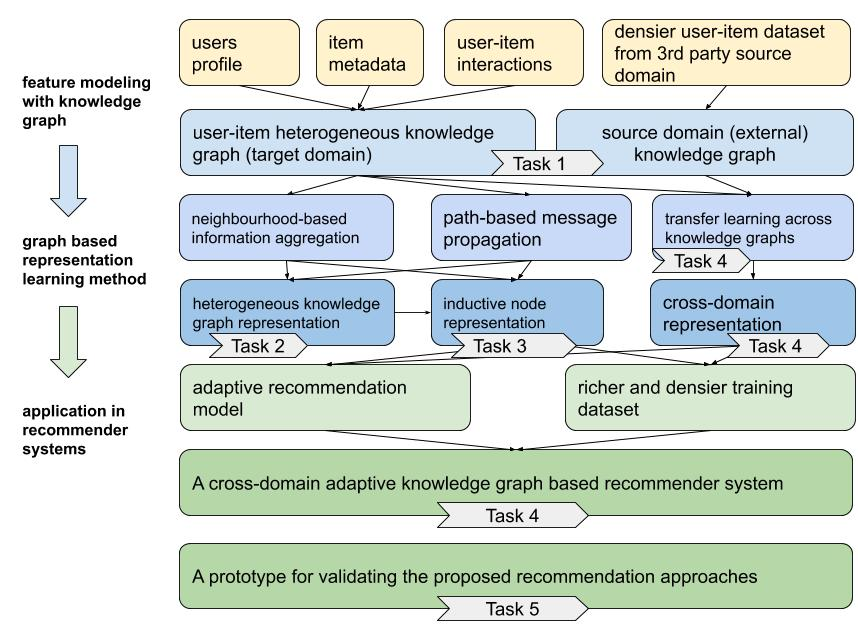
\includegraphics[width=0.98\textwidth]{figs/framework_overview.jpg}
    \caption{framework overview}\label{fig:framework}
\end{figure*}

\subsection{Task 1: Propose a framework that unifies both user/item interactions and side information within single heterogeneous knowledge graph}

For the first task, we form the user-item heterogeneous knowledge graph by unifying user profile, item feature, as well as user-item interactions into a single unified heterogeneous graph.

First, we use side information to crate user and item knowledge graphs. The nodes inside graph can either be item or item features as entities based on data exploration and analytic. Same process applies to the user side, i.e. profile information, such as age, gender, etc. In the end, we would have 2 heterogeneous knowledge graphs, based on users and items respectively as illustrated as G1 and G2 in Figure \ref{fig:meta_task}.
Consequently, we treat user-item interactions as a bipartite graph (as G3 Fig. \ref{fig:meta_task}). As a result, user and item nodes in G1 and G2 are now connected by G3 via "interaction" edges. After this step, we get a unified heterogeneous knowledge graph which contains both user/item feature information as well as interactions.


\begin{figure*}[!ht]
    \centering
    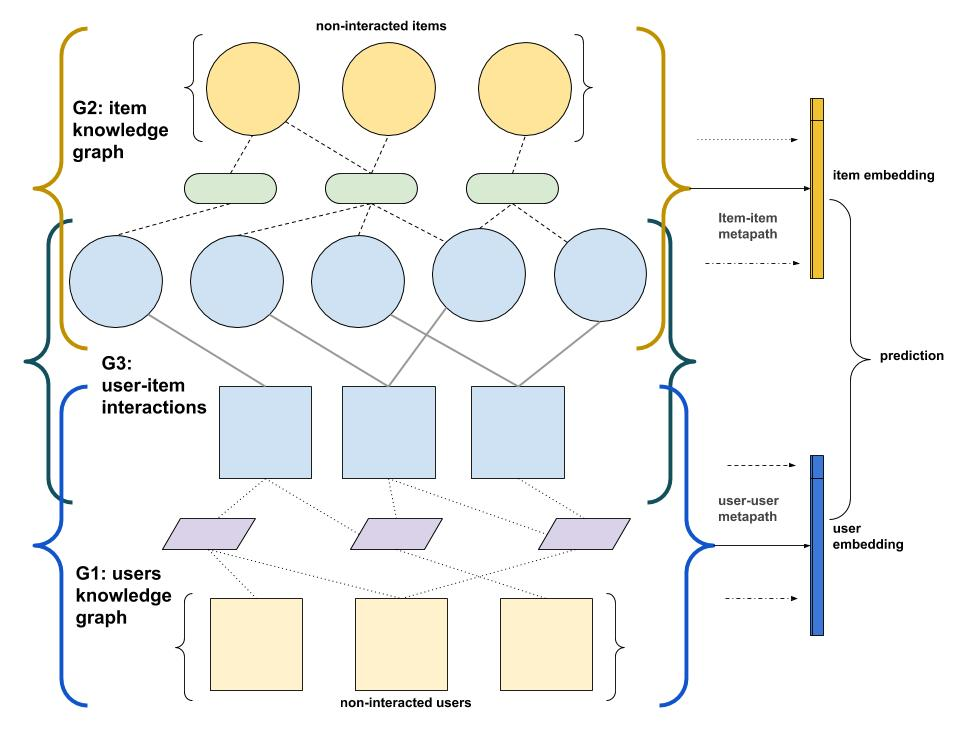
\includegraphics[width=0.98\textwidth]{figs/meta-embedding.jpg}
    \caption{meta-path based interactions via heterogeneous knowledge graph}\label{fig:meta_task}
\end{figure*}

The rich semantic heterogeneous graph structure enables the new data coming to establish relationship via different node and edge types, which also allowing information to be propagated and aggregated through different pathways. 
Intuitively, the node-to-node distance and neighborhood structural comparisons can be both used in measuring user/item similarity for existing or new nodes. In task 3, we would further explore this property to overcome cold start problems and improve recommendation model adaptiveness.


\subsection{Task 2: Build a heterogeneous knowledge graph based method to effectively include non-interacted items}

Most of the recommender systems exclude non-interacted data during training, which limits model prediction ability. In this task, in addition to using direct interactions, we adopt experts knowledge into representation modelling process by defining meta-path connections between nodes. As a result, the model can establish indirect user-item connections via the heterogeneous knowledge graph. For example, \textit{User - Movie} interaction, can be extend to \textit{User - Movie1 - Actor - Movie2}. Consequently, the recommendation model can be benefited from the denser connections inside the heterogeneous graph. One added benefit of such meta-path approach is reducing bias, which happens commonly in the early stage of recommender systems. i.e. When data is not sufficiently available to represent a complete user/item distribution.

On the other hand, incorporating the heterogeneous knowledge graph into a recommender system is not as straight forward as processing tabular dataset. Subsequently, this task transforms node into latent representation through node neighborhood propagation. Collectively, high-order connectivity and node neighborhood structure can be included as part of the representation learning process. So that, side information such as user demographics, item feature representation and node structural information can be transformed into feature vectors holistically by the representative model.

Lastly, we propose a recommendation framework that incorporates the above representation approach. By leveraging factorization machine and path-based similarity within the heterogeneous knowledge graph, both interacted and non-interacted user/item entities can now participate in recommender model training and used for the recommendation predictions. as illustrated in Fig. \ref{fig:meta_task}.

\begin{figure*}[!ht]
    \centering
    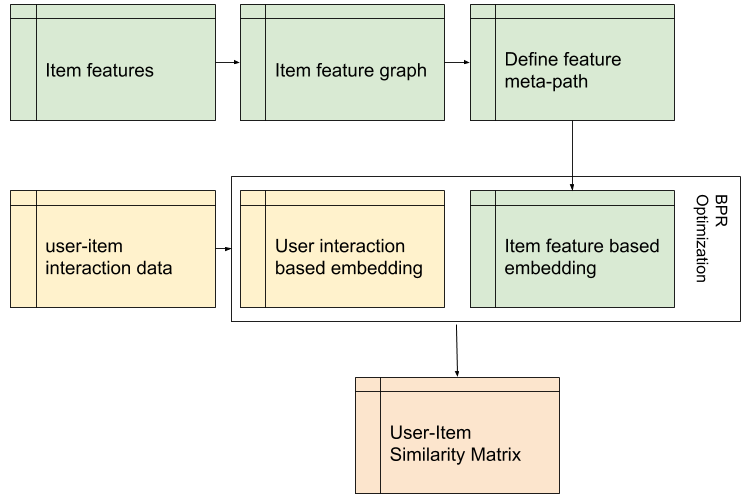
\includegraphics[width=0.95\textwidth]{figs/hkg.png}
    \caption{heterogeneous knowledge graph based recommendation model}\label{fig:meta_task}
\end{figure*}

\subsection{Task 3: Build a adaptive recommendation model via knowledge graph embedding}

\subsubsection*{Step 1: Build a adaptive representation method that is capable of working with unseen user/item data input}

So far, task 1 and task 2 try to alleviate data sparsity problem by forming heterogeneous knowledge graph and establish indirect connections via meta-path. However, our recommendation model is still limited to a static recommendation. i.e. The model is only capable of making predictions on data presented during training phase.

\begin{figure*}[!ht]
    \centering
    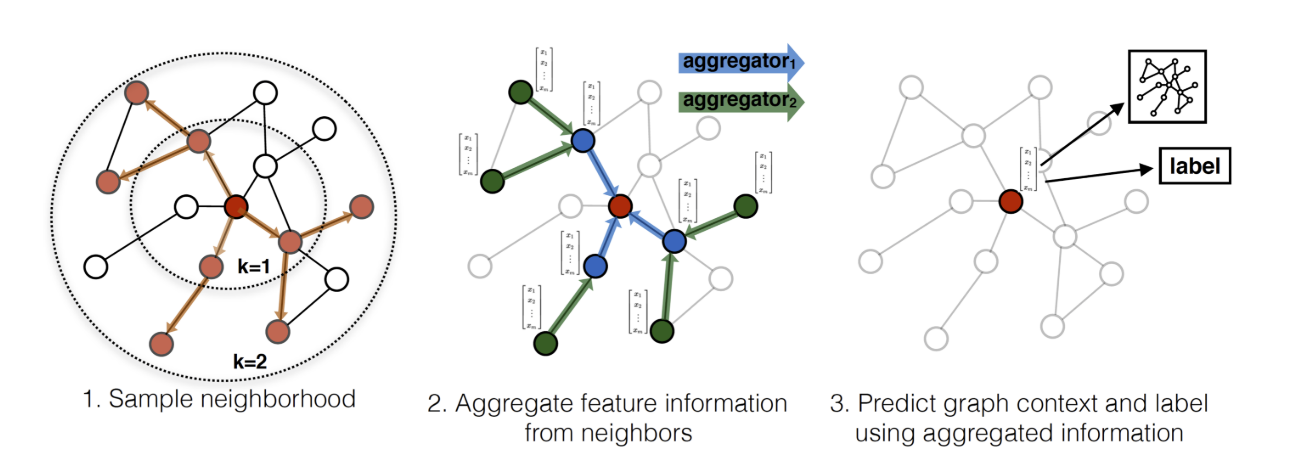
\includegraphics[width=0.95\textwidth]{figs/sagegraph.png}
    \caption{GraphSAGE embedding \citep{hamilton2017inductive}}\label{fig:sagegraph}
\end{figure*}

In order to solve the challenge, the graph convolution network based embedding approach has shown promising results on classification and link prediction problems. \citet{hamilton2017inductive} uses function that generates embeddings by sampling and aggregating features from node neighbors, as shown in Fig. \ref{fig:sagegraph}. In this task, we extend the neighborhood sampling by taking part different meta-path connections into this task. This results a extended message propagation and aggregation rules to sample neighborhood and layers within the knowledge graph. Intuitively, different node relationships would be taken part in the embedding process.

Subsequently, attention approach can be employed. As illustrated in Fig. \ref{fig:gat}, similar to the graph attention network (GAT) approach \citep{velivckovic2017graph}, we apply multi-headed attention mechanisms, which learns different attention coefficients on its neighborhood nodes. The neighborhood nodes here are nodes either directly or indirectly connected via path and meta-paths. Subsequently, the later learnt attention coefficients weights can be used to explain the importance of different meta-paths, which leads to better model interpretability.

\begin{figure*}[!ht]
    \centering
    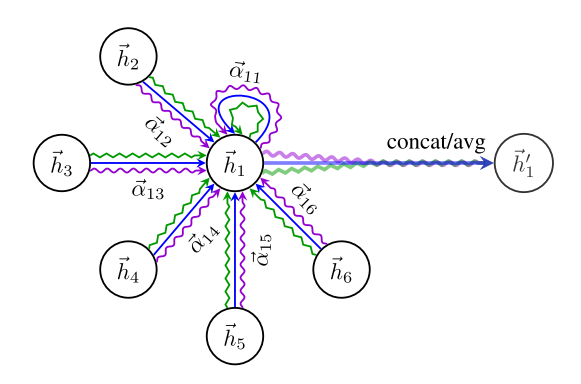
\includegraphics[width=0.6\textwidth]{figs/gat.png}
    \caption{GAT \citep{velivckovic2017graph}}\label{fig:gat}
\end{figure*}

We expect the end result will introduce a general inductive approach, which can efficiently generate node embeddings for unseen data that is not initially included during training.
Experiment will be conducted on different propagation and aggregator approach for node neighborhood sampling. We measure and compare different pooling rules and attention mechanism for the inductive learning step. 

At a high level, this task solves the limitations by inductively generate node embeddings for new data points were not present during training for recommendation predictions. as a result, in the end the final recommendation model are more adaptive to new data input, and more capable of handling prediction in cold start settings.

\subsubsection*{Step 2: Define a recommendation method that leverage inductive representation embedding}
In this task, we aim to optimize node representation inside knowledge graph jointly with collaborative user-item interactions for recommendation objectives.
Based on the findings from step 1, we apply earlier defined propagation rule and aggregator method under following objective function as:

\begin{equation}
    Loss=\min{(L_\text{KGE}+L_\text{FM}+\lambda\|\theta\|^2_2)}
\end{equation}

Where $L_\text{KGE}$ is the optimization target for representation embedding in knowledge graph. Next, we will experiment on different loss option for optimizing recommendation problem. For example, the entity representation can be optimise based on translation principle \citep{lin2017learning}.

\begin{equation}
    L_\text{KGE}=\sum{(h,r,t^+,t^-)} -ln_{sigmoid}(g(h,r,t^-)-g(h,r,t^+))
\end{equation}

While $g(h,r,t)$ is the projected probability from entity $h$ to target entity $t$ propagated via relationship $r$. $^+,^-$ stands for positive and negative samples. Accordingly $L_\text{FM}$ is the BPR \citep{rendle2012bpr} loss for optimizing recommendation objectives.
\begin{equation}
    L_\text{FM} = L_\text{BPR}=\sum{(u,i^+,i^-) \in G_{u,i}} -ln_{sigmoid}(y(u,i^+)-y(u,i^-))
\end{equation}
Where y(u,i) commonly stands for user-item dot product, Intuitively, the its result can be regarded as similarity score.

Lastly, regularization is applied on $\theta$ as model parameters.

Consequently, the trained model entity representation would tailored toward the recommendation objective in a end-to-end fashion.

Experiment and evaluation will be conducted on multiple data conditions, such as sparse dataset, cold stat, zero interaction settings to compare and measure the effectiveness of proposed methods.


\subsection{Task 4: Develop a cross-domains recommender systems based on heterogeneous knowledge graph}

\subsubsection*{Step 1: Develop a knowledge transfer method to improve target domain data sparsity by leveraging source knowledge graph}

In this task, we are going to focus more on transferring knowledge from a different domain, where similar but more abundant information can be learnt and adapted from source domain to target domain for improving both entity representation and recommendation objectives. The research and experiments inside this task will be conducted on 2 different approaches:

\textit{Matrix-based FM method for cross-domain knowledge transfer:}
Matrix-based FM method projects nodes and its neighborhood as one-hot encoding from both source and target knowledge graph into a single matrix. This way, we can treat the matrix containing domain-shared information, such as overlapped user or items. Following up, factorization machine approach is applied on top of the derived matrix. Hence embedding vector can be learnt as $FM(x) = v_x \in R^k$, where $k$ is the vector dimension. Knowledge graph based embedding, which was discussed in task 2 and 3, will be applied here for learning source and target domain-specific representations as $KGE(x)$.
Lastly, concatenation is applied, as, intuitively to combine both domain-shared and domain-specific representations into a single vector.
Additionally, a share $MLP$ function can be applied on both $FM(x)$ and $KGE(x)$ during training phrase. so, the final representation can be denoted as $v_x = [MLP(MF(x));MLP(KEG(x))]$, where $";"$ stand for the concatenation of two node representations.

\textit{GANs-based method for cross-domain knowledge transfer:}
Adversarial domain adaptation technique is another approach we will experiment on transferring knowledge across 2 different domains.
First, we identify common entities, for example shared users or items or their related metadata (such as, item labels, demographics, etc.), to establish connections between source and target domain, and consequently unifying the target and source domain into a single knowledge graph.
Again, knowledge graph embedding will be used for node representation on the unified knowledge graph. Next, a 2 players min-max game are designed for alignment between target and source domains. i.e. a critic will be used for distinguish domain origin based on node representation or interaction connections. A more detail example can be seen in step 2.


\textbf{Step 2: Develop recommendation model that adapt to source domain knowledge graph}

For this task, we extend recommendation model from single domain to multiple domains, in order to further explore on domain adaptation ability by leverage 2 or more knowledge graphs.

Similarly to single domain, we establish richer user-item connections across the source and target domains. Further, common cross-domain entities as described in step 1 can now serve as bridges for unifying and transferring information between 2 knowledge graphs.
For example, when target and source domains shares a common sub-section of users.

Following GANs intuition, we can introduce domain classifier D as critic, a binary classifier, to predict the origin of positive item sample. i.e. is the item belonged to source or target domain based on its representation vector as classifier input. Intuitively, cross graphs node representation and D now can be regarded as 2 players min-max game. It is expected node representation become domain-invariant when reaching equilibrium, i.e. knowledge is transfers across domains, that leads the source and target domain to be aligned. The domain alignment loss can be defined as:

\begin{equation}
    L_\text{DA}(e_s,e_t)=E_{e \in D_s}[log(1-D(e_s))] + E_{e \in D_t}[log(D(e_t))]
\end{equation}

Finally we adjust our cross-domain recommendation objective to as following:

\begin{equation}
    Loss=\min{(L_\text{DA}+L_\text{FM}+\lambda\|\theta\|^2_2)}
\end{equation}



\subsection{Task 5: Build a prototype for validating the proposed recommendation approaches}

The research will be verified from two aspects:
First, verify knowledge graph based recommendation approach using public datasets, such as DBLP Citation Networks, MovieLens data sets. Similarity measure as well as adaptiveness are the core parts of this research, each aspects will be verified accordingly.
Second, the recommendation approach will be used in a real world data sets for solving industry problems. Such as, tourism , job posting and real estate listings where suffers from constant cold start problems. Experiments will be used to further test the effectiveness of the proposed method.

